
\documentclass{IOS-Book-Article}

\usepackage{mathptmx}
\usepackage{rotating,todonotes, xspace}
\usepackage{amssymb}
\usepackage[section]{placeins}
\usepackage{makeidx}  % allows for indexgeneration
\usepackage{algorithm}
\usepackage{algpseudocode}
\usepackage{graphicx}
\usepackage{float}
\usepackage{subcaption}
\captionsetup{compatibility=false}
\usepackage{wrapfig}
\usepackage{array}
\usepackage{multicol}
\usepackage{amsmath}
%\usepackage{times}
%\normalfont
%\usepackage[T1]{fontenc}
%\usepackage[mtplusscr,mtbold]{mathtime}
%
\begin{document}
\begin{frontmatter}              % The preamble begins here.

%\pretitle{Pretitle}
\title{Fault Tolerance and Task Clustering\\
 in Scientific Workflows}
\runningtitle{Fault Tolerant Clustering}
%\subtitle{Subtitle}

\author[A]{{Weiwei} {Chen}%
\thanks{Corresponding Author: Weiwei Chen, University of Southern California, Information Sciences Institute, Marina del Rey, CA, USA; E-mail:
weiweichen@acm.org.}},
\author[A]{Rafael Ferreira de Silva}, 
\author[A]{{Ewa Deelman}}
and 
\author[B]{{Thomas} {Fahringer}}

\runningauthor{W. Chen et al.}
\address[A]{University of Southern California, Information Sciences Institute, Marina del Rey, CA, USA}
\address[B]{University of Innsbruck, Institute for Computer Science, Innsbruck, Austria}

\begin{abstract}
Large scale scientific workflows can be composed of many fine computational granularity tasks. Task clustering has been proven to be an effective method to reduce execution overhead and increase the computational granularity of workflow tasks executing on distributed resources. However, a job composed of multiple tasks may have a greater risk of suffering from failures than a job composed of a single task. Our theoretic analysis and simulation results demonstrate that transient failures can have a significant impact on the runtime performance of scientific workflows that use existing clustering policies that ignore failures. We propose a general task failure modeling framework to address these performance issues. We show the necessity to consider the fault tolerance in the task clustering methods.  We further propose three horizontal methods and one vertical method to improve the runtime performance of executing workflows in dynamic environments. A trace based simulation is performed and it shows that our methods improve the workflow makespan significantly for five important applications.    
\end{abstract}

\begin{keyword}
scientific workflows\sep fault tolerance\sep scheduling\sep locality\sep high availability 
\end{keyword}
\end{frontmatter}

\thispagestyle{empty}
\pagestyle{empty}

\section*{Introduction}


Scientific workflows can be composed of many fine computational granularity tasks and the runtime of these tasks may be even shorter than the system overhead. System overhead is the period time during which miscellaneous work other than the user’s computation is performed. Task clustering \cite{Chen2013, Singh2008, Chen2012, Maheshwari2012, Ferreira-granularity-2013, Integration2012} is a technique that merges several short tasks into a single job such that the job runtime is increased and the overall system overhead is decreased. However, existing clustering strategies ignore or underestimate the impact of the occurrence of failures on system behavior, despite the current and increasing importance of failures in large-scale distributed systems, such as Grids \cite{Bresnahan2011, Deelman2004, Rubing2005}, Clouds \cite{Deelman2008, Berriman2010, Bresnahan2011} and dedicated clusters. Many researchers \cite{Zhang2004, Tang1990, Schroeder2006, Sahoo2004} have emphasized the importance of fault tolerance design and indicated that the failure rates in modern distributed systems are significant. Among all possible failures, we focus on transient failures because they are expected to be more prevalent than permanent failures \cite{Zhang2004}. For example, denser integration of semiconductor circuits and lower operating voltage levels may increase the likelihood of bit-flips when circuits are bombarded by cosmic rays and other particles \cite{Zhang2004}. 

In task clustering, a clustered job consists of multiple tasks. A task is marked as failed (task failure) if is terminated by unexpected events during the computation of this task. If a task within a job fails, this job has a job failure, even though other tasks within this job do not necessarily fail. 
In a faulty environment, there are several options for reducing the influence of workflow failures. First, one can simply retry the entire job when its computation is not successful as in the Pegasus framework \cite{Deelman2004}. However, some of the tasks within the job may have completed successfully and it could be a waste of time and resources to retry all of the tasks. Second, the application process can be periodically checkpointed so that when a failure occurs, the amount of work to be retried is limited. However, the overheads of checkpointing can limit its benefits \cite{Zhang2004}. Third, tasks can be replicated to different nodes to avoid failures that are related to one specific worker node. However, inappropriate clustering (and replication) parameters may cause severe performance degradation if they create long-running clustered jobs. As we will show, a long-running job that consists of many tasks has a higher job failure rate even when the inter-arrival time of failures is long. 

We propose three horizontal methods and one vertical method to improve the existing clustering techniques (with job retry and task replication) in a faulty environment. The first horizontal solution dynamically adjusts the granularity or clustering size (number of tasks in a job) according to the estimated  task failure rate. The second horizontal method retries the failed tasks within a job. And the third horizontal solution is a combination of the first two approaches. The vertical method adjusts the clustering size by dividing a failed job into two even retry jobs to reduce the job failures. We further analyze the runtime performance of combining horizontal methods and vertical methods in different ways. 
In this paper we view the sequence of failure events as a stochastic process and study the distribution of its inter-arrival times, i.e. the time between failures. 

Our work is based on an assumption that the the distribution parameter of the inter-arrival time is a function of the type of task or the node the task is executed on. Samak \cite{Samak2011} et al. have analyzed 1,329 real workflow executions across six distinct applications and concluded that the type and the host id of a job are among the most significant factors that impacted failures. Task type related failure is a type of failure that only occurs to some specific types of tasks. A node failure only occurs to some specific execution nodes. Compared to our prior work in \cite{Chen2012}, we add a parameter learning process to estimate the average task runtime, the average system overhead and the average inter-arrival time of failures. We adopt an approach of prior knowledge based Maximum Likelihood Estimation that has been recently used in machine learning. Knowledge about the parameters are modeled as a distribution with known super-parameters. The distribution of the prior and the posterior are in the same family if the likelihood distribution follows some specific distribution. For example, if the likelihood is a Weibull distribution and we model prior knowledge as an Inverse-Gamma distribution, then the posterior is also an Inverse-Gamma distribution. This simplifies the estimation of parameters and integrates the prior knowledge and runtime datasets gracefully. 

The three horizontal methods were introduced and evaluated in \cite{Chen2012} on two workflows. In this paper, we complement this previous paper by studying (\emph{i}) the performance gain of using three horizontal methods over a baseline execution on a larger set of workflows; (\emph{ii}) the performance impact of the variance of the average task runtime, system overheads and the inter-arrival time of failures; (\emph{iii}) the performance impact of proposed vertical clustering method and its combination with horizontal methods. 

The rest of this paper is organized as follows. Section \ref{sec:related} gives an overview of the related work. Section \ref{sec:models} presents our workflow and failure models. Section \ref{sec:clustering} details our fault tolerant clustering methods. Section \ref{sec:experiments} reports experiments and results, and the paper closes with a discussion and conclusions. 


\section{RELATED WORK}
\label{sec:related}

Failure analysis and modeling \cite{Tang1990} presents system characteristics such as error and failure distribution and hazard rates. Schroeder et al. \cite{Schroeder2006} has studied the statistics of the data, including the root cause of failures, the mean time between failures, and the mean time to repair. Sahoo et al. \cite{Sahoo2004} analyzed the empirical and statistical properties of system errors and failures from a network of heterogeneous servers running a diverse workload. Oppenheimer et al. \cite{Oppenheimer2002} analyzed the causes of failures from three large-scale Internet services and the effectiveness of various techniques for preventing and mitigating service failure. McConnel \cite{McConnel} analyzed the transient errors in computer systems and showed that transient errors follow a Weibull distribution. In \cite{Sun2003, Iosup2008} Weibull distribution is one of the best fit for the workflow traces they used.  Based on these work, we measure the inter-arrival time of failures in a workflow and then provide methods to improve task clustering.  

Overhead analysis~\cite{Ostberg2011, Prodan2008} is a topic of great interest in the Grid community. Stratan et al.~\cite{Stratan2008} evaluate in a real-world environment Grid workflow engines including DAGMan/Condor and Karajan/Globus. Their methodology focuses on five system characteristics: overhead, raw performance, stability, scalability, and reliability. They pointed out that head node consumption should not be negligible and the main bottleneck in a busy system is often the head node. Prodan et al.~\cite{Prodan2008} offered a complete Grid workflow overhead classification and a systematic measurement of overheads. In Chen et al.~\cite{Chen2011}, we extended~\cite{Prodan2008} by providing a measurement of major overheads imposed by workflow management systems and execution environments and analyzed how existing optimization techniques improve runtime by reducing or overlapping overheads. The prevalent existence of system overheads is an important reason why task clustering provides significant performance improvement for workflow-based applications. In this work, we aim to further improve the performance of task clustering in a faulty environment. 

Machine learning has been used to predict execution time \cite{Rubing2009, 1015660, 1542747} and system overheads~\cite{Chen2011}, and develop probability distributions for transient failure characteristics. Duan et.al. \cite{Rubing2009} used Bayesian network to model and predict workflow task runtimes. The important attributes (such as the external load, arguments etc. ) are dynamically selected by the Bayesian network and fed into a radial basis function neural network to make further predictions. In our paper, we reuse the knowledge (the family distribution) gained from prior work on failure analysis, overhead analysis and task runtime analysis. We then use prior knowledge based Maximum Likelihood Estimation to integrate both the knowledge and runtime feedbacks and adjust the estimation accordingly. 

The low performance of \emph{fine-grained} tasks is a common problem in widely distributed platforms where the scheduling overhead and queuing times at resources are high, such as Grid and Cloud systems. Several works have addressed the control of task granularity of bag of tasks. For instance, Muthuvelu et al.~\cite{Muthuvelu2005} proposed a clustering algorithm that groups bag of tasks based on their runtime---tasks are grouped up to the resource capacity. Later, they extended their work~\cite{4493929} to determine task granularity based on task file size, CPU time, and resource constraints. Recently, they proposed an online scheduling algorithm~\cite{Muthuvelu2010} that groups tasks based on resource network utilization, user's budget, and application deadline. Ng et al.~\cite{Keat2006} and Ang et al.~\cite{Ang2009} introduced bandwidth in the scheduling framework to enhance the performance of task scheduling. Longer tasks are assigned to resources with better bandwidth. Liu and Liao~\cite{Liu2009} proposed an adaptive fine-grained job scheduling algorithm to group fine-grained tasks according to processing capacity and bandwidth of the current available resources. Although these techniques significantly reduce the impact of scheduling and queuing time overhead, they did not consider fault tolerance.

Task granularity control has also been addressed in scientific workflows. For instance, Singh et al.~\cite{Singh2008} proposed a level- and label-based clustering. In level-based clustering, tasks at the same level can be clustered together. The number of clusters or tasks per cluster are specified by the user. In the label-based clustering, the user labels tasks that should be clustered together. Although their work considers data dependencies between workflow levels, it is done manually by the users, which is prone to errors. Recently, Ferreira da Silva et al.~\cite{Ferreira-granularity-2013} proposed task grouping and ungrouping algorithms to control workflow task granularity in a non-clairvoyant and online context, where none or few characteristics about the application or resources are known in advance. Their work significantly reduced scheduling and queuing time overheads, but did not consider fault tolerance.


\section{Design and Models}
\label{sec:models}



\subsection{Workflow Model}


\label{sec:model}


A workflow is modeled as a directed acyclic graph (DAG), where each node in the DAG often represents a workflow task ($t$), and the edges represent dependencies between the tasks that constrain the order in which tasks are executed. Dependencies typically represent data-flow dependencies in the application, where the output files produced by one task are used as inputs of another task. Each task is a computational program and a set of parameters that need to be executed. 
%Figure~\ref{fig:model_odag} (left) shows an illustration of a DAG composed of four tasks. 
This model fits several workflow management systems such as Pegasus~\cite{Deelman2004}, Askalon~\cite{Fahringer2005}, and Taverna~\cite{Oinn2004}. In this paper, we assume there is only one execution site with multiple compute resources, such as virtual machines on the clouds. 


Figure~\ref{fig:model_system} shows a typical workflow execution environment. The submit host prepares a workflow for execution (clustering, mapping, etc.), and worker nodes, at an execution site, execute jobs individually. The main components are introduced below:

\begin{figure}[!htb]
\centering
  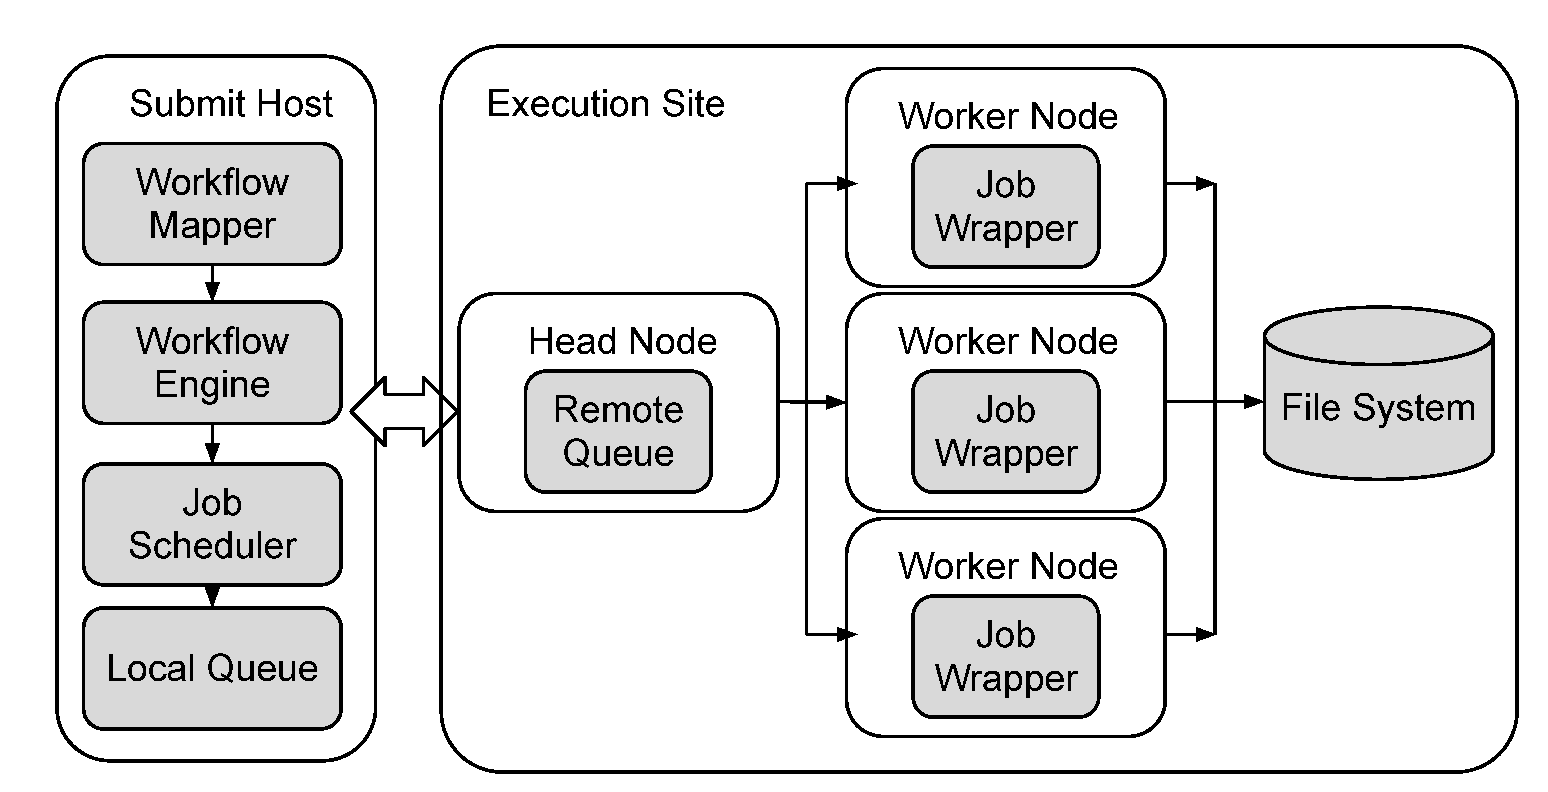
\includegraphics[width=0.95\linewidth]{figure2.eps}
  \caption{A workflow system model.}
  \label{fig:model_system}
\end{figure}

\paragraph{Workflow Mapper} Generates an executable workflow based on an abstract workflow~\cite{Deelman2004} provided by the user or workflow composition system. It also restructures the workflow to optimize performance and adds tasks for data management and provenance information generation. In this work, the workflow mapper is used to merge small tasks together into a job such that system overheads are reduced (\textbf{task clustering}). A job is a single execution unit in the workflow execution systems and is composed of one or more tasks. 

\paragraph{Workflow Engine} Executes jobs defined by the workflow in order of their dependencies. Only jobs that have all their parent jobs completed are submitted to the Job Scheduler. The Workflow Engine relies on the resources (compute, storage, and network) defined in the executable workflow to perform computations. The elapsed time from when a job is released (all of its parents have completed successfully) to when it is submitted to the job scheduler is denoted as the workflow engine delay. %The workflow engine delay is usually configured by users to assure that the entire workflow scheduling and execution system is not overloaded. 

\paragraph{Job Scheduler and Local Queue} Manage individual workflow jobs and supervise their execution on local and remote resources. The elapsed time from when a task is submitted to the job scheduler to when it starts its execution in a worker node is denoted as the queue delay. It reflects both the efficiency of the job scheduler and the resource availability. 

\paragraph{Job Wrapper} Extracts tasks from clustered jobs and executes them at the worker nodes. The clustering delay is the  elapsed time of the extraction process.

\begin{figure}[!htb]
	\centering
	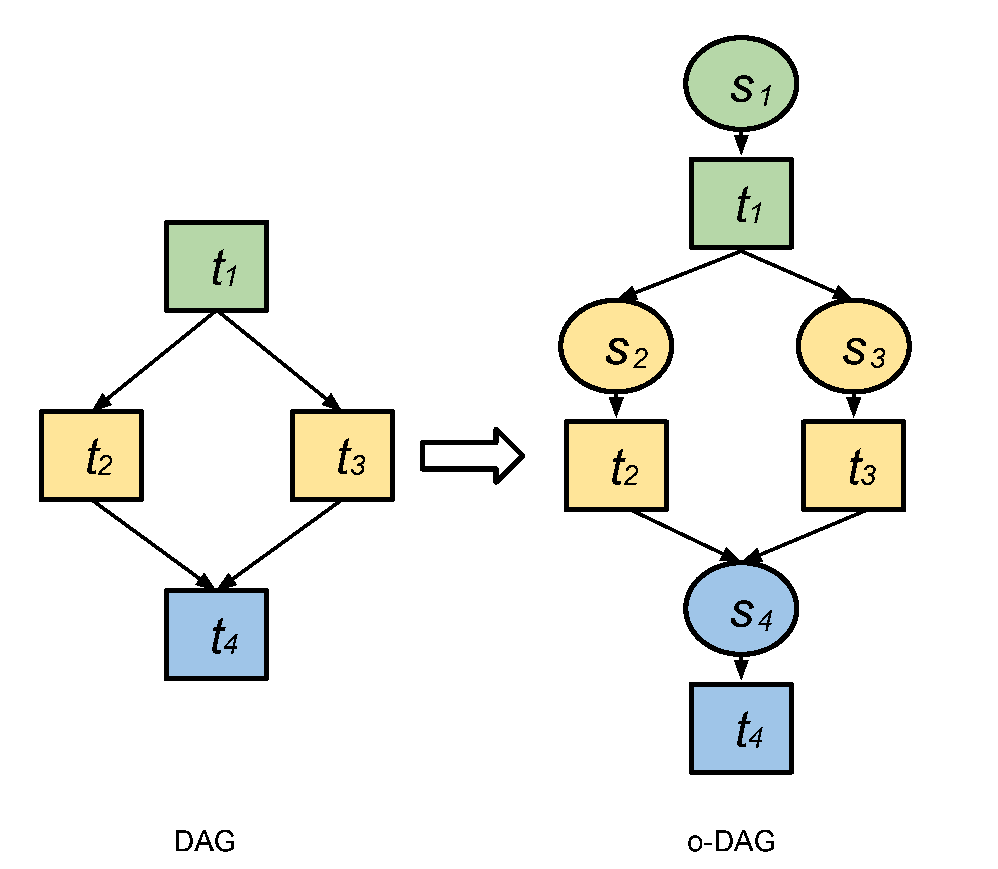
\includegraphics[width=0.7\linewidth]{figure1.eps}
	\captionof{figure}{Extending DAG to o-DAG. `s' denotes a system overhead. }
	\label{fig:model_odag}
\end{figure}

We extend the DAG model to be overhead aware (o-DAG). System overheads play an important role in workflow execution and constitute a major part of the overall runtime when tasks are poorly clustered~\cite{Chen2011}. Figure~\ref{fig:model_odag} shows how we augment a DAG to be an o-DAG with the capability to represent system overheads ($s$) such as workflow engine and queue delays. In addition, system overheads also include data transfer delay caused by staging-in and staging-out data. This classification of system overheads is based on our prior study on workflow analysis~\cite{Chen2011}. 

With an o-DAG model, we can explicitly express the process of task clustering. In this paper, we address task clustering horizontally and vertically. \textbf{Horizontal Clustering} (HC) merges multiple tasks that are at the same horizontal level of the workflow, in which the horizontal level of a task is defined as the longest distance from the entry task of the DAG to this task. \textbf{Vertical Clustering} (VC) merges tasks within a pipeline of the workflow. Tasks at the same pipeline share a single-parent-single-child relationship, which means a task $t_a$ is the unique parent of a task $t_b$, which is the unique child of $t_a$. 

Figure~\ref{fig:model_hc} shows a simple example of how to perform HC, in which two tasks $t_2$ and $t_3$, without a data dependency between them, are merged into a clustered job $j_1$. A job $j$ is a single execution unit composed by one or multiple task(s). Job wrappers are commonly used to execute clustered jobs, but they add an overhead denoted by the clustering delay $c$. The clustering delay measures the difference between the sum of the actual task runtimes and the job runtime seen by the job scheduler. 
After horizontal clustering, $t_2$ and $t_3$ in $j_1$ can be executed in sequence or in parallel, if parallelism in one compute node is supported. In this work, we consider sequential executions only. Given a single resource, the overall runtime for the workflow in Figure~\ref{fig:model_hc} (left) is $runtime_l= \sum_{i=1}^{4}(s_i+t_i)$, and the overall runtime for the clustered workflow in Figure~\ref{fig:model_hc} (right) is $runtime_r=s_1+t_1+s_2+c_1+t_2+t_3+s_4+t_4$.  $runtime_l > runtime_r$ as long as $c_1 < s_3$, which is the case in many distributed systems since the clustering delay within a single execution node is usually shorter than the scheduling overhead across different execution nodes. 

\begin{figure}[!htb]
\centering
 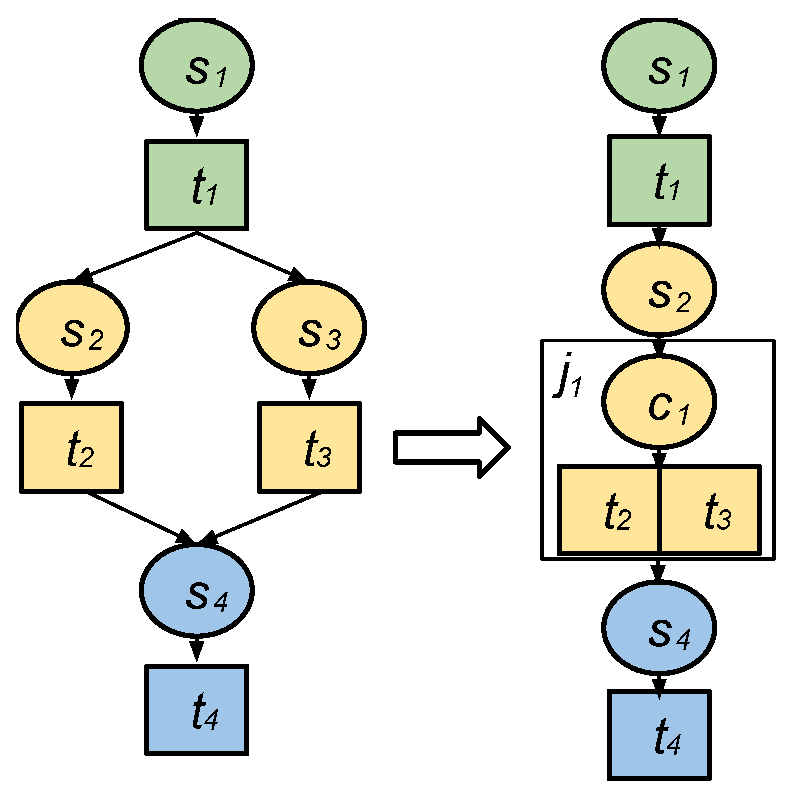
\includegraphics[width=0.55\linewidth]{figure3.eps}
  \captionof{figure}{An example of horizontal clustering (color indicates the horizontal level of a task).}
  \label{fig:model_hc}
\end{figure}

\begin{figure}[!htb]
\centering
 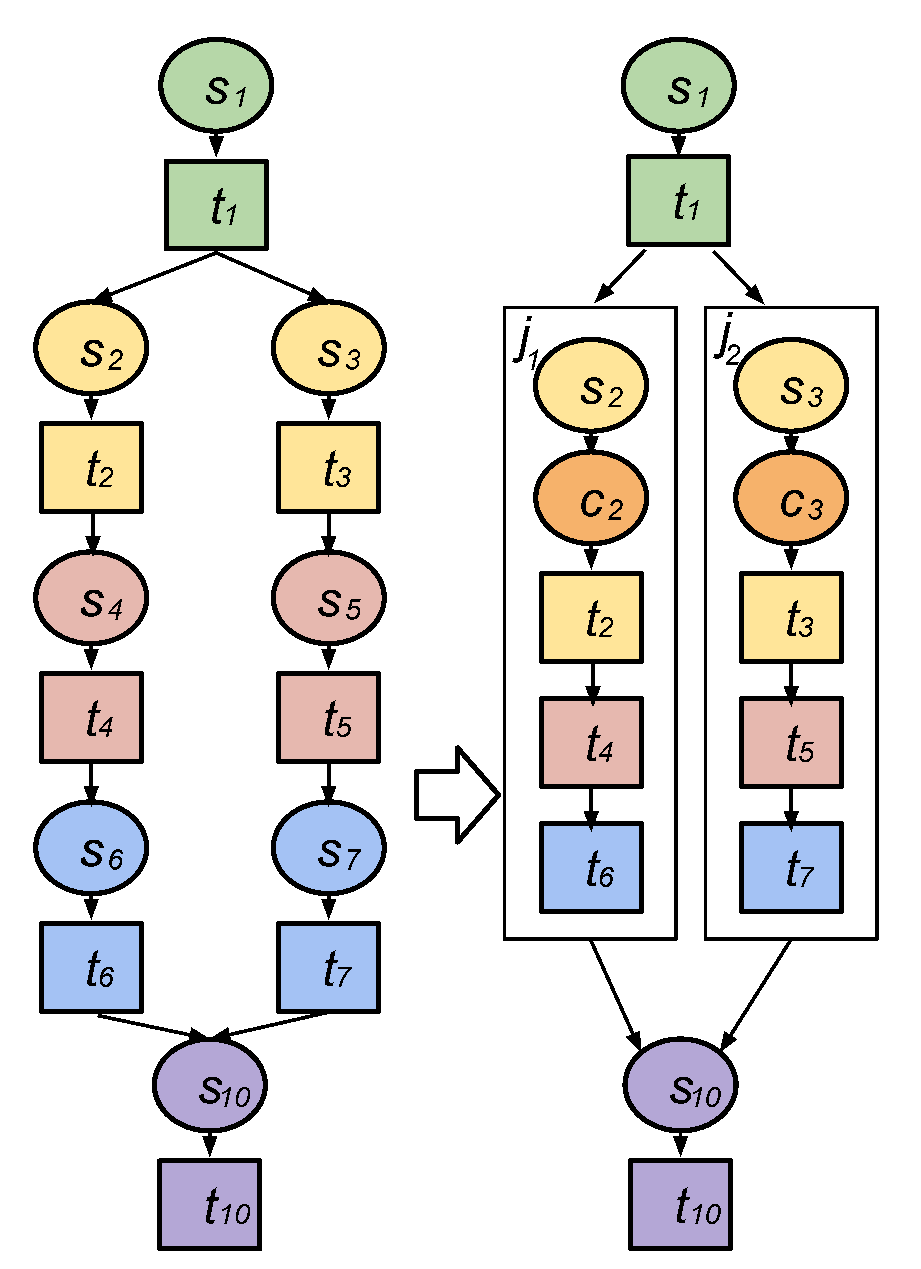
\includegraphics[width=0.6\linewidth]{figure4.eps}
  \captionof{figure}{An example of vertical clustering.}
  \label{fig:model_vc}
\end{figure}

Figure~\ref{fig:model_vc} illustrates an example of vertical clustering, in which tasks $t_2$, $t_4$, and $t_6$ are merged into $j_1$, while tasks $t_3$, $t_5$, and $t_7$ are merged into $j_2$. Similarly, clustering delays $c_2$ and $c_3$ are added to $j_1$ and $j_2$ respectively, but system overheads $s_4$, $s_5$, $s_6$, and $s_7$ are removed. 


In task clustering, the clustering size ($k$) is an important parameter to influence the performance. We define it as the number of tasks in a clustered job. For example, the $k$ in Figure~\ref{fig:model_hc} is 2. The reason why task clustering can help improve the performance is that it can reduce the scheduling cycles that workflow tasks go through since the number of jobs has decreased. The result is a reduction in the scheduling overhead and possibly other overheads as well \cite{Chen2011}. Additionally, in the ideal case without any failures, the clustering size is usually equal to the number of all the parallel tasks divided by the number of available resources. Such a naïve setting assures that the number of jobs is equal to the number of resources and the workflow can utilize the resources as much as possible. However, when transient failures exist, we claim that the clustering size should be set based on the failure rates especially the task failure rate. Intuitively speaking, if the task failure rate is high, the clustered jobs may need to retry more times compared to the case without clustering. Such performance degradation will counteract the benefits of reducing scheduling overheads. In the rest of this paper, we will show how to adjust $k$ based on the estimated parameters of average task runtime $t$, average system overhead $s$ and the inter-arrival time of task failures $\gamma$. 

\subsection{Task Failure Model}

%For system overhead $p(X|\theta)$, we assume it follows an Weibull distribution with known shape $\kappa=0.78$. When $x>0$, the PDF of $p(x|\theta, \kappa)$ is

%\begin{equation}
%f(x|\theta, \kappa)=\frac{\kappa}{\theta} (\frac{x}{\theta})^{\kappa-1}e^{-(x/\theta)^{\kappa}}  \nonumber
%\end{equation}

In our prior work \cite{Chen2011}, we have verified that system overheads $s$ fits gamma or Weibull distribution better than the other two distributions (Exponential and Normal). Schroeder et. al. \cite{Schroeder2006} have verified the inter-arrival time of task failures fits a Weibull distribution with a shape parameter of 0.78 or a gamma distribution better than lognormal and exponential distribution. In \cite{Sun2003, Iosup2008} Weibull distribution is one of the best fit for the workflow traces they used.  Without loss of generality, we choose Weibull distribution to represent the distribution of task runtime ($t$), system overhead ($s$) and the inter-arrival times of failures ($\gamma$).  $s$ is a random variable representing the system overheads. $t$ is a random variable representing the task runtime. 

In Bayesian probability theory, if the posterior distribution $p(\theta|D, a, b)$ are in the same family as the prior distribution $p(\theta|a, b)$, the prior and the posterior are then called conjugate distributions, and the prior is called a conjugate prior for the likelihood function. For example, the Inverse Gamma family is conjugate to itself (or self-conjugate) with respect to a Weibull likelihood function: if the likelihood function is Weibull, choosing a Inverse Gamma prior over the mean will ensure that the posterior distribution is also Inverse Gamma. This simplifies the estimation of parameters since we can reuse the prior work from other researchers on the failure analysis and performance analysis. 

The conjugate pair of Weibull distribution is Inverse Gamma distribution, which means if the prior follows an Inverse Gamma distribution with parameters (the scale parameter $a$ and the shape parameter $b$), the posterior also follows an Inverse Gamma distribution with parameters (the scale parameter $a+n$ and the shape parameter $\displaystyle b+\sum_{i=1}^n{x_i^\kappa}$). The Maximum Likelihood Estimation  (MLE) of posterior is $\displaystyle\frac{b+\displaystyle\sum_{i=1}^n{x_i^\kappa}}{a+n+1}$. The understanding of the MLE has two folds: initially we do not have any data and thus the MLE is $\displaystyle\frac{b}{a}$, which means it is determined by the prior knowledge; when $n\to\infty$, the MLE is $\displaystyle\frac{\displaystyle\sum_{i=1}^n{x_i^\kappa}}{n+1}\to\bar{x}$, which means it is determined by the observed data and it is close to the average of the observed data. 

After we observe data $D$ (runtime, failure, overhead data collected during the execution of workflows), we compute the posterior distribution of $\theta$:

\begin{eqnarray}
	\displaystyle  
	p(\theta|X, a, b)&=&\frac{p(\theta|a, b)\times p(X|\theta)}{p(X|a, b)}\nonumber  \\
	&\propto&p(\theta|a, b)\times p(X|\theta)\nonumber 
\end{eqnarray}

$X$ could be $s$, $t$ or $\gamma$. $p(\theta|X,a, b)$ is the posterior that we aim to compute. $p(\theta|a, b)$ is the prior, which we have already known from previous work. $p(X|\theta)$ is the likelihood. We only need to know its shape parameter instead of its scale parameter, which reduces the work to estimate its scale parameter. 

\begin{figure*}[!htb]
\centering
  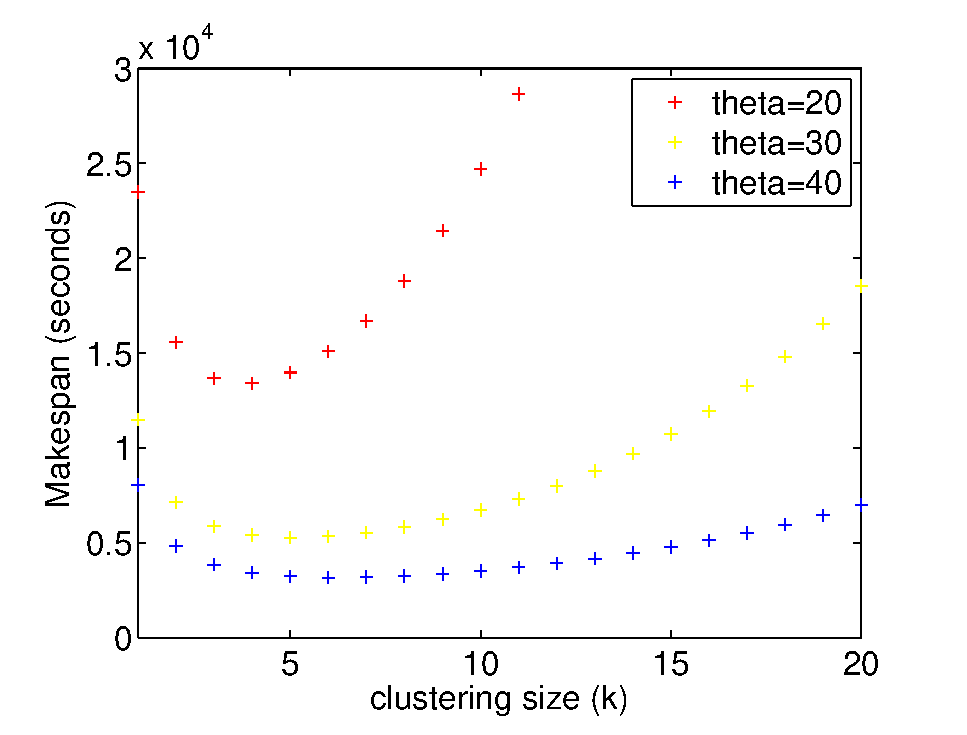
\includegraphics[width=0.95\linewidth]{figure5.eps}
  \caption{Makespan with different clustering size. ($n=1000$, $r=20$, $t=5$ sec, $s=50$ sec)}
  \label{fig:model_makespan}
\end{figure*}

\begin{figure*}[!htb]
\centering
  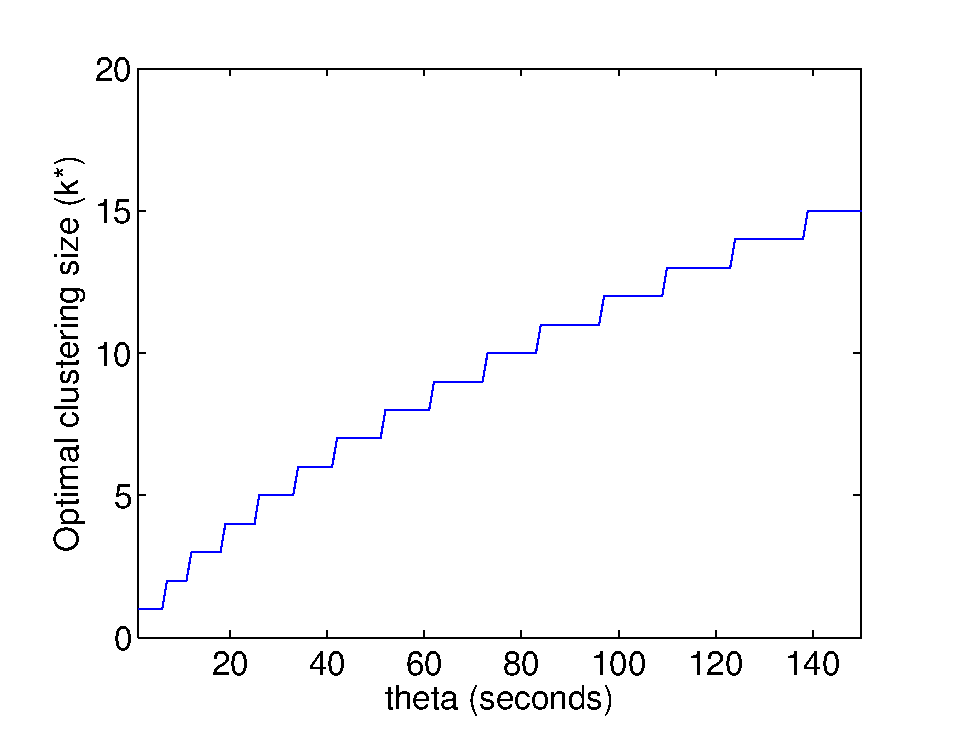
\includegraphics[width=0.95\linewidth]{figure6.eps}
  \caption{Optimal clustering size (k*) with different  $\theta$ ($n=1000$, $r=20$, $t=5$ sec, $s=50$ sec)}
  \label{fig:model_size}
\end{figure*}

We have already assumed the task runtime, system overhead and inter-arrival time between failures are a function of task types. Since in scientific workflows, tasks at the different level (the deepest depth from the entry task to this task) are usually of different type, we model the runtime level by level. Given $n$ independent tasks at the same level, $n$ resources, the estimated average task runtime $t$, the estimated average system overhead $s$, and the estimated inter-arrival time of failures $\gamma$, we aim to reduct the overall runtime $M$ of completing these tasks by adjusting the clustering size $k$ (the number of tasks in a job). 
$M$ includes the runtime of the clustered job and its subsequent retry jobs if the first try fails. For a clustered job, let the expectation of retry times be $N$. The process to run and retry a job is a Bernoulli trial with only two results: success or failure. Once a job fails, it will be retried until it is eventually completed successfully since we assume the failures are transient. By definition we have, 
\begin{eqnarray}
\displaystyle
N=\frac{1}{1-F(kt+s)}=\frac{1}{e^{-(\displaystyle\frac{kt+d}{\theta})^{\kappa}}} \nonumber
\end{eqnarray}

$F(x)$ is the CDF of $t$, $s$ or $\gamma$ under known shape parameter $\kappa$ and estimated scale parameter $\theta$. 

We define a clustered job succeeds only if all of its tasks succeed. We assume that $n \gg r$, but $n/k$ is not necessarily much larger than $r$ since $k$ could be very large. Normally at the beginning of workflow execution, $n/k > r$, which means there are more clustered jobs than available resources. To try all $n$ tasks once, irrespective of whether they succeed or fail, one needs approximately $\displaystyle \frac{n}{rk}$ execution cycle(s) since at each execution cycle we can execute at most $r$ jobs. Therefore, the time to execute all n tasks once is $\displaystyle\frac{n(kt+s)}{rk}$. And the time to complete them successfully in a faulty environment is $\displaystyle\frac{Nn(kt+s)}{rk} $ since each job requires $N$ retries on average.  

On the other side, at the end of the workflow execution, since n is decreasing with the process of workflow, it is possible that $\displaystyle \frac{n}{k} < r$, which means there are fewer jobs than the available resources. One needs just one execution cycle to execute these tasks once. The time to complete all $n$ tasks successfully is $N(kt+d)$. 

In summary, the estimated overall runtime is, 

\begin{equation} 
\label{eq:jfm}
M=
\begin{cases}
\cfrac{n(kt+s)}{rk}{e^{-(\cfrac{kt+s}{\theta})^{\kappa}}}, & \text{if } \cfrac{n}{k}\geq r \\
(kt+s){e^{-(\cfrac{kt+s}{\theta})^{\kappa}}}, & \text{else}
\end{cases}
\end{equation}
Let $k^*$ is the optimal clustering size and $M^*$ is the minimal runtime of these $n$ tasks.  Figure~\ref{fig:model_makespan} shows the three examples of $M$ using a low task failure rate ($\theta=40$s), a medium task failure rate ($\theta=30$s) and a high task failure rate ($\theta=20$s). Other parameters are $n=1000$, $t=5$ sec, $s=50$ sec, and $r=20$. These parameters are close to the level of mProjectPP in the Montage workflow that we simulate in Section \ref{sec:experiments}. It is difficult to find a analytical solution of $k^*$. However, there are a few constraints that can simplify the estimation of $k^*$: (\emph{i}) $k$ can only be integers in practice; (\emph{ii}) $M$ is continuous and has one minimal when $\displaystyle 1<k<\frac{n}{r}$. We use Newton's method to find the minimal $M$ and the corresponding $k$. Figure \ref{fig:model_size} shows the relationship between the optimal clustering size ($k^*$) and the estimated inter-arrival time between failures ($\gamma$), which is a non-decreasing function. It is consistent with our expectation since the longer the inter-arrival time of failures is, the lower the task failure rate is. With a lower task failure rate, a larger $k$ assures that we reduce system overheads without retrying many times.  


%We performed a parameter searching study, where we first estimate the upper bound of $k$ as $\displaystyle\frac{n}{r}$ since after $M$ is a monotonic increasing function of $k$ when $k\geq\displaystyle\frac{n}{r}$, and the lower bound of $k$ as 1 for simplicity. Data points are divided into ten chunks and then we sample one data point from each chunk. We then select the chunk that has the lowest makespan and set the new upper and lower bounds as the borders of the selected chunk, respectively. These steps are repeated until the upper and lower bounds have converged into a data point. 



From this theoretic analysis, we conclude that (\emph{i}) the longer the inter-arrival time of failures is, the better runtime performance the task clustering has; (\emph{ii}), adjusting the clustering size according to the detected inter-arrival time can improve the runtime performance. 

\section{Fault Tolerant Clustering}
\label{sec:clustering}

As indicated in Section \ref{sec:model}, inappropriate clustering may increase the makespan of a workflow. To improve the fault tolerance from the point of view of clustering, we propose three horizontal methods: Dynamic Clustering (\emph{DC}), Selective Reclustering (\emph{SR}) and Dynamic Reclustering (\emph{DR}) and one vertical clustering method: Binary Reclustering (\emph{BR}). 

A.	Dynamic Clustering (DC)

Dynamic Clustering adjusts the clustering size according to the task failure rates measured from jobs that have already been completed, either successfully or failed. Currently we use the average value of task failure records. 
 
Failure records contain the information about the number of failed tasks, the type of tasks, the resource id, and a timestamp. The type of tasks is used to detect the task specific failures and the resource id is used to detect location specific failures. Then we calculate the average task failure rate and the average job failure rate. Figure 5 shows an example where the initial clustering size is 4 and thereby there are four tasks in a clustered job at the beginning. During execution, three out of these tasks fail. TFM suggests an optimal clustering size to be 2, then this job will be split into two clustered jobs while each has two tasks and the two clustered jobs are then submitted for retry.  DC is not aware that there are only three failed tasks. 

According to Eq. (4), an estimation of the minimal makespan in DC can be simplified as:
                                             (5)
B.	Selective Reclustering (SR)
In DC, one knows the average task failure rate but the information about which tasks have failed is not available. In practice, it may be hard to identify the failed tasks, but if it is supported, we can further improve the performance with Selective Reclustering that selects the failed tasks in a clustered job and clusters them into a new clustered job, or treats them individually. SR is different to the naïve job retry in that the latter method retries all tasks of a failed job even though some of the tasks have succeeded. SR requires collecting the task ids in failure records. 
Figure 6 shows an example of SR. At the beginning, there are four tasks and three of them have failed. One task succeeds and exits. Only the three failed tasks are merged again into a new clustered job and the job is retried. This approach does not intend to adjust the clustering size, although the clustering size will be smaller and smaller naturally after each retry since there are less and less tasks in a clustered job. In this case, the clustering size has reduced from 4 to 3.
 
Figure 6	Selective Reclustering.
C.	Dynamic Reclustering (DR)
Selective Reclustering does not analyze the failure rate rather, it uses a natural way to reduce the clustering size if the failure rate is too high. However, it requires a special ability to select the failed tasks, while DC does not. We then propose the third method, Dynamic Reclustering, which is a combination of SR and DC to see whether using both strategies can improve workflow performance. In DR, only failed tasks are merged into new clustered jobs and the clustering size is also adjusted according to the detected task failure rates.
 
Figure 7	Dynamic Reclustering
Figure 7 shows the steps of DR. At the last scheduling cycle, three tasks within a clustered job have failed. Therefore we have only three tasks to retry and further we need to adjust the clustering size (in this case it is 2) according to the task failure rate. 

\section{Experiments and Discussions}
\label{sec:experiments}

In this section, we evaluate our methods with two workflows, whose runtime information is gathered from a real execution traces. The simulation-based approach allows us to control system parameters such as task failure rate in a continuous way so as to clearly demonstrate the performance of the algorithms. Our methods can also be applied to real workflow management systems as long as they support failure logging. 

\subsection{Experiments Setup and Workflows Used}
We use a real trace of the Montage workflow [1] and the Periodogram application to evaluate our models and optimization methods. The reason why we chose Montage and Periodogram is that they represent two different types of workflows. As shown in Figure 1, Montage has complex data dependencies between tasks/jobs while Periodogram is simply a bag-of-tasks. Montage is an astronomy application used to construct large image mosaics of the sky.  Runtime data are collected from real runs under the Pegasus Workflow Management System (WMS) [7]. We ran the Montage workflow with a size of 8 degree squares of sky. The workflow has 10,422 tasks and 57GB of overall data. The workflow was run on a cluster with 20 nodes. The Periodogram application is also developed by IPAC (Caltech) to identify periodic signals from light curves that arise from transiting planets and stellar variability. The Periodogram workflow we ran has ~216,600 tasks and 19GB input data. The Periodogram workflow has only one level of tasks. 
With these runtime information and file size, we use CloudSim [6] to simulate the workflows in a controlled environment.  CloudSim is a framework for modeling and simulation of cloud computing infrastructures and services. Internally, workflow execution is divided into four steps: first, the workflow engine releases tasks based on the dependencies between tasks; second, the clustering engine merges the released tasks into jobs; third, these jobs are submitted to the job scheduler and are matched with resources based on different criteria specified by users; fourth, each job is executed by a worker node that has input files and executable files available. Each workflow was simulated at least 100 times to assure that standard deviation in the workflow makespan is less than 10%. 
To make the simulation consistent with the real results in Pegasus WMS, we modified CloudSim to execute our simulations.  Figure 8 shows the system overview of our simulation. The Workflow Engine manages tasks and jobs based on their dependencies between jobs to assure that a job may only be released when all of its parent jobs have completed successfully. It also loads workflow logs that are gathered and reconstructed from prior runs. The Clustering Engine merges tasks on the same horizontal level into clustered jobs according to the suggested clustering size (k*). The Job Scheduler is revised to match jobs to the most reliable worker nodes and avoid or even skip a worker node that has too many failures compared to others. The Failure Generator is added to generate task failures according to the specified average task failure rate. The Failure Monitor serves as an agent that suggests clustering size based on the estimation of the task failure rate, the type of task, and the node to be matched. Based on this information, the Clustering Engine will adjust the clustering size in DC or DR approaches.
 
Figure 8	 System Overview
\subsection{Dynamic Performance}
To evaluate the performance of TFM and DC, we first simulated the Montage workflow with a fixed task failure rate (α = 0.002).  
 
Figure 9	clustering size
Figure 9 shows the difference between the actual clustering size and the suggested clustering size at each scheduling interval. The scheduling cycle is a period when the Workflow Engine releases tasks that are ready to run and the Clustering Engine merges these tasks along with tasks that have failed. Montage has three major horizontal levels of tasks that require clustering, which are mProjectPP, mDiffFit, and mBackground. At the beginning, the Failure Monitor does not have enough failure records to identify the task failure rate. We adopt a risky strategy in that the initial clustering size is set to be n/r so that all tasks will be tried once at the beginning. That is why the actual clustering size at cycle 1 is approximately 25 and then it falls down quickly. After passing 5, the actual k and the suggested k overlap with each other since the Failure Monitor has collected enough data to adapt to the faulty environment. From the cycle 4 to 14, the workflow is mainly executing mDiffFit, and during that time the suggested k and actual k fall down to 6 eventually since our model requires some time to run jobs first and then predict the task failure rate. The suggested k and the actual k for mBackground fall to 3 quickly since at this step the prediction of task failure rate is already stabilized. The reason that each type of task has different clustering sizes is that they have different runtime on average. 
  Figure 9 also reminds us that the actual k is sometimes smaller than the suggested k, which has been explained in cycle 1 to 3. At cycle 3, the actual k is smaller than the suggested k because the Clustering Engine does not have sufficient tasks to be clustered since most tasks are completed. We will address this issue and improve the performance in Section IV.D. 

\subsection{Performance of different Optimization Methods}
TABLE I	WORKFLOW MAKESPAN (MONTAGE, UNIT: SECOND) 
α	Optimization Methods
	NOOP	DC	SR	DR
0.002	9827	9010	8168	8633
0.004	11390	9224	8174	8687
0.006	13625	9430	8181	8771
0.008	16989	9590	8191	8818
0.01	22026	9709	8202	8856
0.02	169075	10218	8242	8930
0.04	44099753	10853	8316	9153
0.06	N/A 	11488	8387	9344
0.08	N/A	11951	8461	9734
TABLE II	WORKFLOW MAKESPAN (PERIODOGRAM, UNIT: SECOND) 
α	Optimization Methods
	NOOP	DC	SR	DR
0.002	17180	15141	13824	15052
0.004	18197	15272	13853	15106
0.006	18930	15360	13883	15130
0.008	19344	15464	13911	15159
0.01	19668	15566	13941	15176
0.02	19889	16081	14086	15363
0.04	21407	17141	14376	15712
0.06	24147	18283	14681	16109
0.08	26597	19511	15010	16478
We compare the workflow makespan when running the workflow with DC, SR, DR and No Optimization (NOOP) with task failure rate in a range between 0.2% and 8%. Researchers [14] show that a transient failure rate is not usually more than 10%; otherwise such a system does not have much practical usage. If the task failure rate is lower than 0.1%, one doe not need to apply our methods. 

 
Figure 10	Workflow Makespan (Periodogram)
We present the workflow makespan improvement of Montage in TABLE I and the results of Periodogram in TABLE II and Figure 10. Both improvements are significant particularly with SR since it is able to identify the failed tasks. Even though DC has optimized the clustering size according to a prediction of task failure rate, the jobs to be retried still contain both failed tasks and successful tasks. DR performs better than DC as we have expected. Both SR and DR exclude the successful tasks and only retry the failed tasks within a job. However, they require the ability to identify tasks that have failed in a clustered job, which DC does not. These tables also show that the improvement is more significant when the task failure rate is higher, which is consistent to our previous claim. Particularly for Montage, we reduce the growth of makespan from a near-exponential increase (in NOOP) to a near-linear increase, which is a giant leap for task clustering. What is more, SR performs better than DR in the two workflows, which shows that there is still a gap between dynamically adjusting the clustering size based on task failure rate and naturally retrying failed tasks. This might be caused by the simplification of our models and it suggests us to investigate the performance issues further.


\section{Future Work}

In the future, we plan to apply our work to a real world framework---the Pegasus Workflow Management System and to evaluate the performance with more applications. We will also examine failures with different distribution, such as for example Weibull.  We will further evaluate the robustness of our methods to the variance of failure patterns, runtime, and overhead. The gap between DC and SR indicates that there is still space for further improvement in the approach of dynamically adjusting the workflow task clustering size. 

\section{ACKNOWLEDGMENT}
This work is supported by NFS under grant number IIS-0905032. We thank Gideon Juve, Karan Vahi, Mats Rynge and Rajiv, Mayani for their help. 


\bibliographystyle{elsarticle-num}
\bibliography{biblio}

\end{document}
